% generated by scripts/pkl_to_latex.py
% source PKL : uscan_v1_L8_Ne8_t1_mode-uniform_nmin2_solver-gcg_full_restarts8_iter200_kmax4_tol1em09_U1to20_N20-d03a74da789e.pkl
% scan type  : uscan
% state      : gs
% quantity   : purity
% requires   : \usepackage{pgfplots} \pgfplotsset{compat=1.18}
% colours match the matplotlib PDF (tab10 cycle)
\definecolor{gmeC0}{HTML}{1F77B4}
\definecolor{gmeC1}{HTML}{FF7F0E}
\definecolor{gmeC2}{HTML}{2CA02C}
\definecolor{gmeC3}{HTML}{D62728}
\definecolor{gmeC4}{HTML}{9467BD}
\definecolor{gmeC5}{HTML}{8C564B}
\definecolor{gmeC6}{HTML}{E377C2}
\definecolor{gmeC7}{HTML}{17BECF}

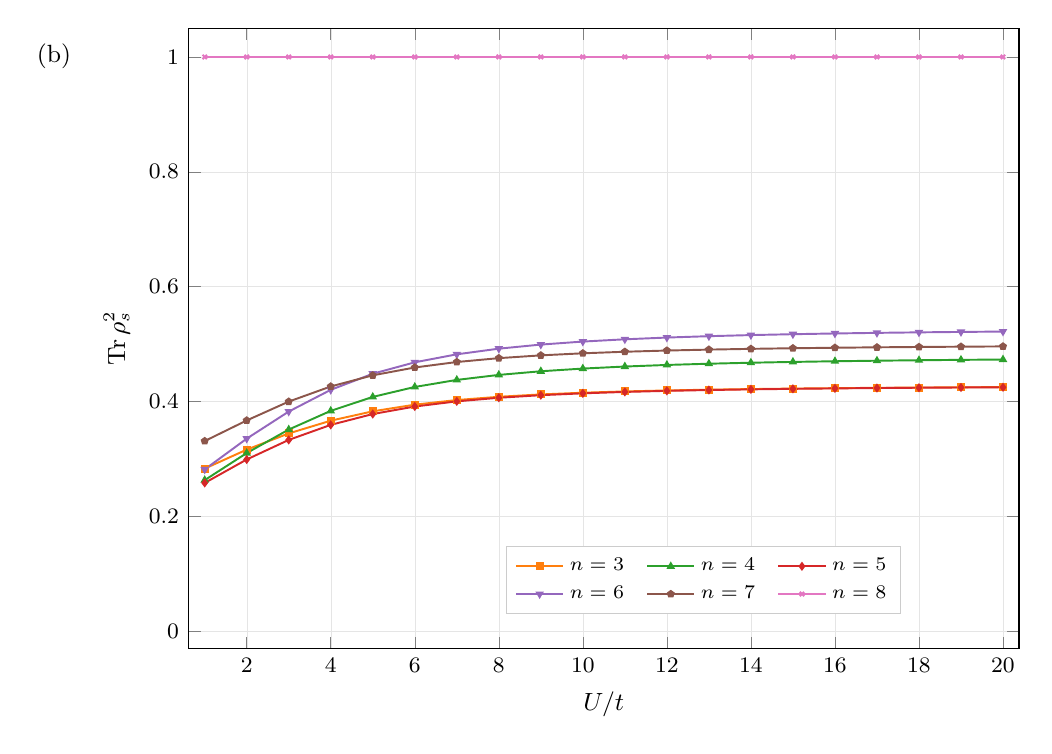
\begin{tikzpicture}
  \begin{axis}[
    width=\columnwidth,
    height=0.78\columnwidth,
    xlabel={$U/t$},
    ylabel={$\mathrm{Tr}\,\rho_s^2$},
    grid=both,
    grid style={line width=.1pt, draw=gray!20},
    tick label style={font=\footnotesize\rmfamily, /pgf/number format/fixed},
    label style={font=\small\rmfamily},
    scaled ticks=false,
    legend style={font=\scriptsize\rmfamily, draw=gray!40, at={(0.5,1.03)}, anchor=south, /tikz/every even column/.append style={column sep=6pt}},
    legend cell align={left},
    legend columns=3,
    ymin=-0.03,
    ymax=1.05,
    xmin=0.62,
    xmax=20.38,
    legend style={at={(0.620,0.110)}, anchor=center, fill=white},
    after end axis/.append code={\node[anchor=east, font=\small\rmfamily] at (axis description cs:-0.13,0.954) {(b)};},
  ]
    \addplot[color=gmeC1, mark=square*, mark size=1.1pt, line width=0.7pt] coordinates {
        (1,0.283101) (2,0.316165) (3,0.344373) (4,0.366544)
        (5,0.382879) (6,0.394436) (7,0.402509) (8,0.40819)
        (9,0.412262) (10,0.415247) (11,0.417485) (12,0.419201)
        (13,0.420541) (14,0.421607) (15,0.422468) (16,0.423172)
        (17,0.423756) (18,0.424245) (19,0.424659) (20,0.425013)
    };
    \addlegendentry{$n=3$}
    \addplot[color=gmeC2, mark=triangle*, mark size=1.1pt, line width=0.7pt] coordinates {
        (1,0.263016) (2,0.310158) (3,0.351091) (4,0.383677)
        (5,0.407936) (6,0.425285) (7,0.437547) (8,0.44628)
        (9,0.452613) (10,0.457304) (11,0.460856) (12,0.4636)
        (13,0.465759) (14,0.467486) (15,0.468888) (16,0.47004)
        (17,0.470999) (18,0.471805) (19,0.472489) (20,0.473074)
    };
    \addlegendentry{$n=4$}
    \addplot[color=gmeC3, mark=diamond*, mark size=1.1pt, line width=0.7pt] coordinates {
        (1,0.258129) (2,0.299) (3,0.333057) (4,0.359251)
        (5,0.378117) (6,0.391203) (7,0.400207) (8,0.406476)
        (9,0.410937) (10,0.414191) (11,0.416624) (12,0.418483)
        (13,0.419934) (14,0.421086) (15,0.422016) (16,0.422776)
        (17,0.423406) (18,0.423934) (19,0.42438) (20,0.424761)
    };
    \addlegendentry{$n=5$}
    \addplot[color=gmeC4, mark=triangle*, mark size=1.1pt, mark options={rotate=180}, line width=0.7pt] coordinates {
        (1,0.281632) (2,0.335276) (3,0.382457) (4,0.420268)
        (5,0.4483) (6,0.468182) (7,0.482118) (8,0.491975)
        (9,0.499082) (10,0.504323) (11,0.508276) (12,0.51132)
        (13,0.51371) (14,0.515617) (15,0.517162) (16,0.51843)
        (17,0.519484) (18,0.520369) (19,0.521118) (20,0.521759)
    };
    \addlegendentry{$n=6$}
    \addplot[color=gmeC5, mark=pentagon*, mark size=1.1pt, line width=0.7pt] coordinates {
        (1,0.331081) (2,0.366968) (3,0.399786) (4,0.42615)
        (5,0.445535) (6,0.459185) (7,0.468717) (8,0.475451)
        (9,0.480308) (10,0.483894) (11,0.486602) (12,0.48869)
        (13,0.490331) (14,0.491642) (15,0.492705) (16,0.493579)
        (17,0.494305) (18,0.494916) (19,0.495433) (20,0.495875)
    };
    \addlegendentry{$n=7$}
    \addplot[color=gmeC6, mark=x, mark size=1.1pt, line width=0.7pt] coordinates {
        (1,1) (2,1) (3,1) (4,1)
        (5,1) (6,1) (7,1) (8,1)
        (9,1) (10,1) (11,1) (12,1)
        (13,1) (14,1) (15,1) (16,1)
        (17,1) (18,1) (19,1) (20,1)
    };
    \addlegendentry{$n=8$}
  \end{axis}
\end{tikzpicture}
